\section{\Sys Design}
\label{sec:methodology}

In this section, we outline the architecture of our system, \Sys, which comprises five principal modules. The first module, the \textit{Provenance Graph Constructor}, operates on each client machine, transforming audit logs into a provenance graph. The second module, \textit{Semantic Featurization}, focuses on encoding semantic attributes from audit logs into feature vectors, which aids in the training of the client-specific \gnnshort models. This process utilizes word2vec models, each individually trained on its respective client's logs.

The third module, \textit{Semantic Vectors Harmonization}, is tasked with merging these individual word2vec models into a unified global model. This is achieved using a trusted utility server and encryption techniques to safeguard sensitive model data. 

Following this, the \textit{Federated Graph Learning Module} undertakes the task of training \gnnshort models on each client machine, utilizing the harmonized semantic features. Once the individual client models are trained, they engage in a federated learning process facilitated by the central server. In this process, each client transmits its model to the server, where the federated averaging algorithm is applied to amalgamate these models into a singular, comprehensive global model. This consolidated model is then dispatched back to the clients for further application and analysis.

Finally, the \textit{Anomaly Detection Module} utilizes the aggregated global model for local anomaly detection on each client machine. Figure \ref{arch} illustrates the overarching architecture of \Sys, with a more comprehensive explanation provided in the following subsections:

\begin{figure}[t!]
  \centering
  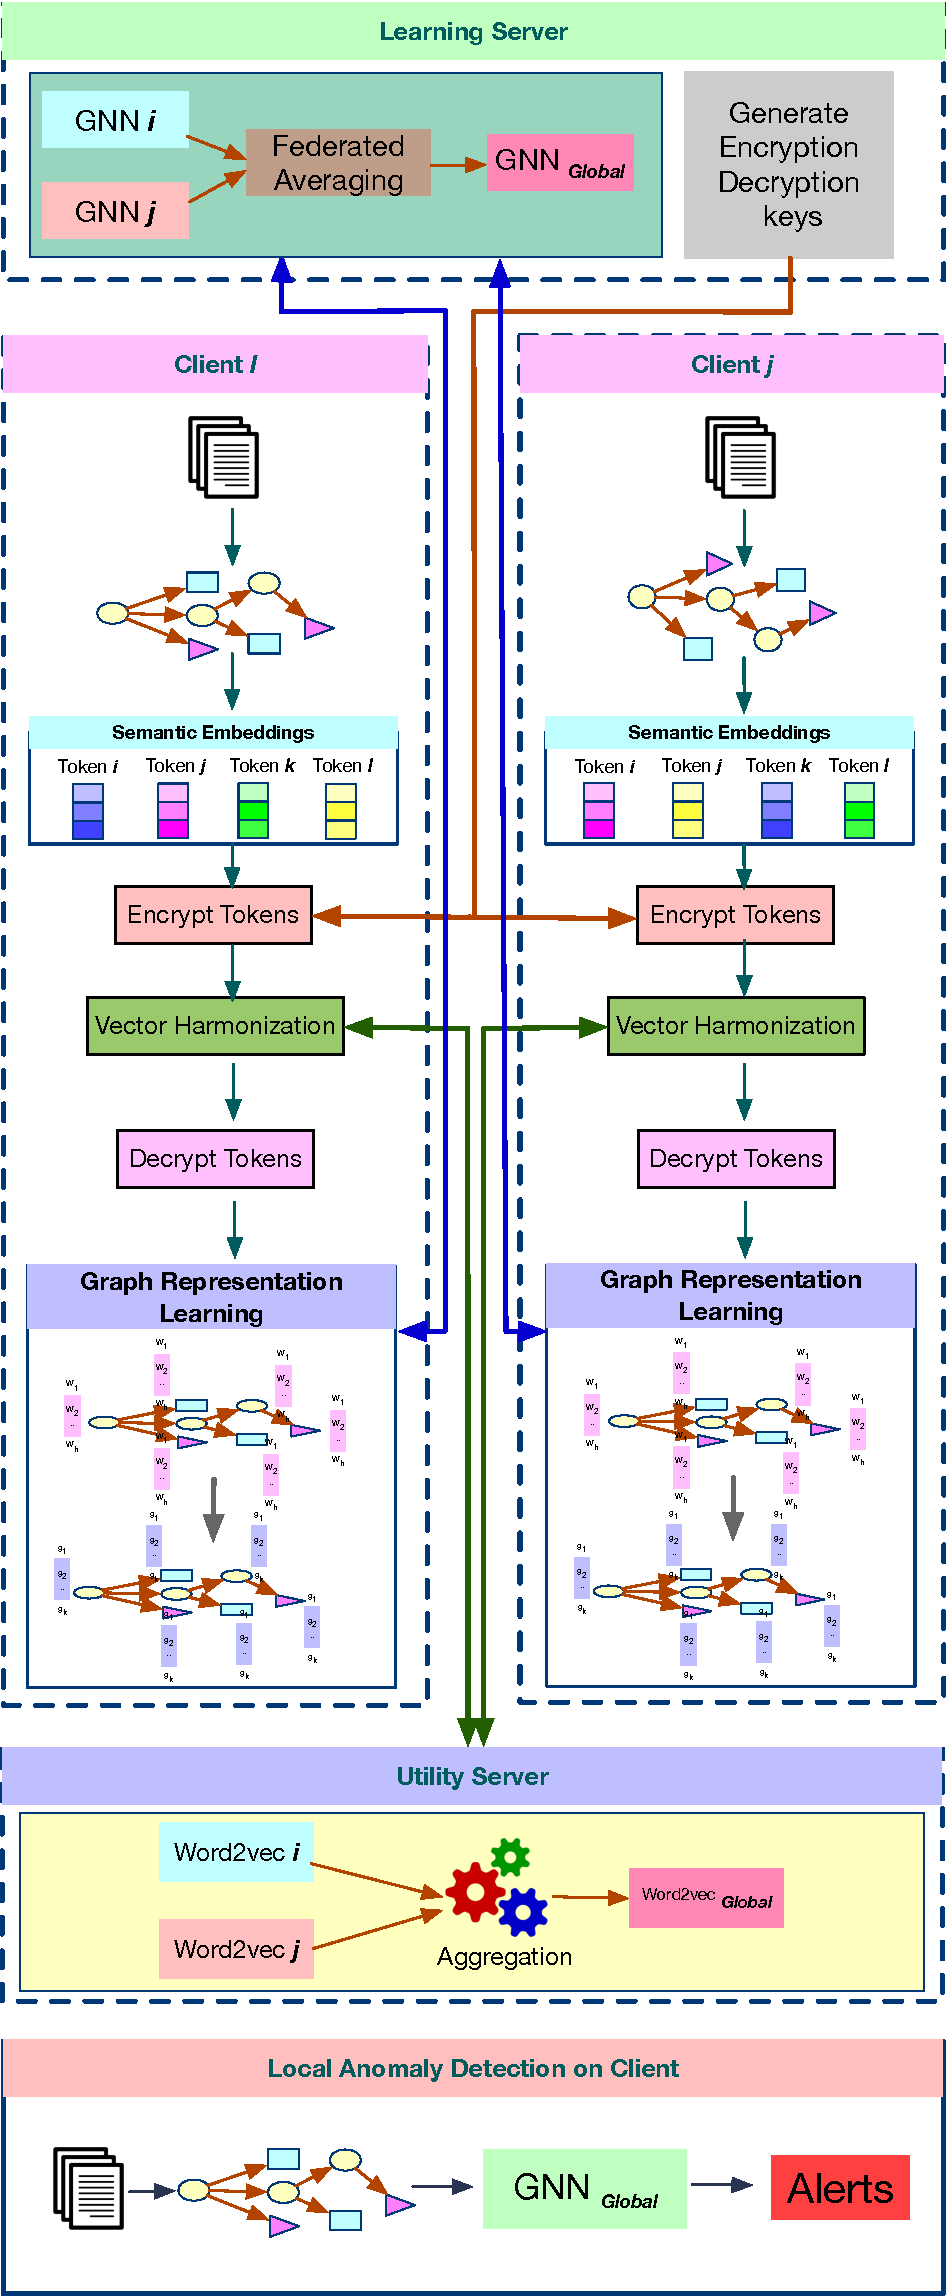
\includegraphics[width=0.45\textwidth]{fig/arch.pdf}
  \caption{High Level Architecture of \Sys.}%\wajih{Please reduce the different number of colors you are using in this diagram. They are distracting. Also, it is not clear from this diagram what is the order of operation. Maybe you need to put numbers on the edges. Or you need to make it from left to right to show which thing will happen first and then second and so on.}}
  \vspace{-3ex}
  \label{fig:arch}
\end{figure}

\subsection{Provenance Graph Constructor} 
\Sys harnesses audit logs to create a system provenance graph. It operates on each client machine, utilizing their local system logs for graph construction. Key operating systems, such as Linux and Windows, are equipped with built-in mechanisms, namely the Linux Audit system and Windows Event Tracing, for log collection. These logs offer comprehensive insights into the interactions among different system entities, documenting activities ranging from process executions and file operations to network connections. Utilizing this information, \Sys assembles a graph where nodes represent system entities like processes, files, and sockets. The edges of this graph correspond to events, predominantly identified by syscalls, that occur between these entities. In addition, \Sys augments each node with detailed attributes, including process names, command lines, file names, and network IP addresses. This enrichment of node attributes significantly bolsters our system's proficiency in differentiating between nodes with analogous graph structures.

\subsection{Semantic Featurization}
\wajih{use word2vec macro.}
% This module processes the provenance graph generated from audit logs by transforming node attributes into feature vectors for the graph learning phase. Existing systems like Flash have demonstrated the effectiveness of using semantic node attributes to enhance detection performance. Building on this approach, we employ a word2vec language model to encode these attributes into vector format. Each client independently trains a word2vec model using their local system logs. However, before these models can be utilized to encode text attributes, they must be merged across client machines to form a unified model. This unification is crucial; without it, each client would produce differing feature vectors for identical inputs. Such variability would undermine the consistency of client-based \gnnshort models and diminish the effectiveness of the federated averaging technique.

This module processes the provenance graph generated from audit logs by transforming node attributes into feature vectors for the graph learning phase. Systems like Flash have demonstrated the effectiveness of using semantic node attributes to enhance detection performance. Building on this approach, we employ a word2vec language model to encode these attributes into vector format, \(\mathbf{v}\), where each attribute \(a\) is transformed into a vector \(v_a\). Each client independently trains a word2vec model using their local system logs. The transformation of an attribute \(a\) into a vector by the word2vec model can be represented as:

\[
v_a = \text{word2vec}(a)
\]

However, before these models can be utilized to encode text attributes, they must be merged across client machines to form a unified model. This unification is crucial; without it, each client would produce differing feature vectors, \(v_a^i\), for identical inputs, where \(i\) indicates the client. The variability in feature vectors, \(\{v_a^1, v_a^2, \ldots, v_a^N\}\), for the same attribute \(a\) across \(N\) clients, would undermine the consistency of client-based GNN models. To ensure uniformity, the feature vectors for overlapping attributes must be averaged across clients, forming a single unified vector for each attribute:

\[
\bar{v}_a = \frac{1}{N} \sum_{i=1}^{N} v_a^i
\]

Such averaging ensures consistency in the feature representation, enhancing the effectiveness of the federated averaging technique by maintaining uniformity in the input space for the GNN models across all clients.


\subsection{Semantic Vectors Harmonization}
This module integrates individual client word2vec models into a unified model for use across all clients. The word2vec model functions as a key-value store, with vocabulary tokens as keys, \(k\), and their corresponding vector representations as values, \(v_k\). To combine these models, we calculate the average vector of overlapping tokens from all client machines, creating a central model. The mathematical representation for averaging vectors of a token \(k\) across \(N\) clients is given by:

\[
\bar{v}_k = \frac{1}{N} \sum_{i=1}^{N} v_{k,i}
\]

where \(\bar{v}_k\) is the averaged vector for token \(k\), and \(v_{k,i}\) is the vector representation of token \(k\) from the \(i\)-th client model.

However, transferring tokens—containing sensitive data like process names, file names, and IP addresses—to a central server could breach user privacy. To mitigate this, we employ a trusted utility server. Initially, the central server distributes an encryption key, \(E\), and a decryption key, \(D\), pair to each client. Clients then encrypt their word2vec model tokens using the encryption key:

\[
E(v_{k}) = v_{k}^{'}
\]

and send them to the utility server. This server merges the encrypted models and dispatches the unified model back to the clients, who decrypt it using the decryption key:

\[
D(v_{k}^{'}) = v_{k}
\]

This procedure ensures that neither the central server nor the utility server can access the actual token information, assuming no collusion between the two servers. The process is explained in detailed in algorithm~\ref{alg:secure_integration_averaging_word2vec}

\begin{algorithm}[h]
  \scriptsize
  \DontPrintSemicolon
  \SetKwInOut{Input}{Inputs}
  \SetKwInOut{Output}{Output}
  \Input{Client Word2Vec models $\{M_1, M_2, \ldots, M_N\}$ encrypted with key $E$; Encryption key $E$; Decryption key $D$.}
  \Output{Encrypted unified Word2Vec model $U'$ sent to clients.}
  \BlankLine
  \tcc{Distribute encryption and decryption keys to each client.}
  \ForEach{client $C_i$}{
    Send $E$ and $D$ to $C_i$\\
  }
  \tcc{Clients encrypt their model tokens.}
  \ForEach{client model $M_i$}{
    $M_i' \leftarrow$ EncryptModelTokens($M_i$, $E$) \tcc*{Encrypt tokens using $E$.}
    Send $M_i'$ to Utility Server\\
  }
  \tcc{Utility server merges encrypted models.}
  $TokenVectors \leftarrow$ InitializeEmptyDictionary()\\
  $TokenCounts \leftarrow$ InitializeEmptyDictionary()\\
  \ForEach{encrypted model $M_i'$}{
    \ForEach{token $t$ in $M_i'$}{
      $Vector \leftarrow M_i'[t]$\\
      \eIf{$TokenVectors$.HasKey($t$)}{
        $TokenVectors[t] \leftarrow TokenVectors[t] + Vector$\\
        $TokenCounts[t] \leftarrow TokenCounts[t] + 1$\\
      }{
        $TokenVectors[t] \leftarrow Vector$\\
        $TokenCounts[t] \leftarrow 1$\\
      }
    }
  }
  \tcc{Average the vectors for overlapping tokens.}
  \ForEach{token $t$ in $TokenVectors$.Keys()}{
    $TokenVectors[t] \leftarrow TokenVectors[t] / TokenCounts[t]$\\
  }
  $U' \leftarrow$ NewModel($TokenVectors$, $EncryptedTokens$) \tcc*{Constructing a new unified model.}
  \ForEach{client $C_i$}{
    Send $U'$ to $C_i$\\
  }
  \BlankLine
  \Return{Harmonized model $U'$ has been dispatched to all clients.}\\
  \BlankLine
  \caption{Secure Integration and Averaging of Word2Vec Models}
  \label{alg:secure_integration_averaging_word2vec}
\end{algorithm}

\subsection{Federated Graph Learning}
The module performs graph representation learning in a federated manner. It includes a central server responsible for initializing a global \gnnshort model with random weights, which is then sent to all clients. These clients use their local provenance graphs and semantic feature vectors to train the \gnnshort model in an unsupervised way, following a training method similar to Flash. The \gnnshort model's objective is to classify each node entity into its corresponding type. After training their models, the clients send them back to the central server. The server applies the federated averaging algorithm to merge these models into a single global model. The server aggregates parameters from $N$ client models to update the global model as follows:
\[
\bar{w} = \frac{1}{N} \sum_{k=1}^{N} w_k
\]

where:
\begin{itemize}
    \item $\bar{w}$ is the aggregated global model parameter.
    \item $N$ is the number of client models.
    \item $w_k$ is the parameter from the $k$-th client model.
\end{itemize}

This formula averages the parameters of all client models, forming the global model update. The process is repeated for a set number of rounds, determined by a hyperparameter, and concludes when there is no further reduction in training loss. Algorithm~\ref{alg:federated_learning} explains this process in detail.

\subsection{Anomaly Detection}
\Sys employs an advanced methodology akin to systems like Flash and \threatrace, focusing on identifying irregular nodes through the comparison of their expected and observed types. This approach is grounded in a detailed analysis of both the surrounding structures and inherent properties of the nodes, with the aim to define normal pattern baselines for various node types. Typically, entities with malicious intentions display neighborhood configurations and characteristics deviating from these established norms. In operational phases, the detection of anomalies that diverge from the pre-established node distribution patterns often results in their misclassification. The emergence of nodes misclassified in the system's output is indicative of potential security issues. To regulate the frequency of alerts, we have implemented a threshold parameter, denoted as $T$. This parameter sets a limit on the likelihood of a classification being considered valid. A higher value of this parameter implies stronger confidence in the prediction, increasing the probability of identifying anomalies.

\wajih{Whrere is the part about local differential privacy? We should have something about that in design section.}


% \subsection{Provenance Graph Constructor}
% Our approach starts by converting system logs into provenance graphs through a three-step process. Initially, the system, \Sys, processes system logs like Windows Event Logs or Linux Audit Logs, which are composed of host event details including process activities, file interactions, and network engagements. \Sys works with batches of audit logs, utilizing a sliding window technique to create the provenance graph. This graph consists of two kinds of nodes: process nodes and object nodes. The object nodes represent various system entities such as files, network streams, modules, and other system components. The connections between these nodes are marked with labels indicating the event type, elucidating the cause-and-effect relationship among the connected nodes and the event's timestamp. Additionally, these nodes are equipped with attributes like process identifiers, command lines, file paths, IP addresses, port details, and module paths, offering additional insights and specifics.

% \subsection{Semantic Vectors Harmonization}
% \wajih{You need to add formalism in this subsection overall. If there is a Math related to Harmonization add that. Look into the Flash paper -- we gave so much internal details about the algorithms. }
% Our system employs the word2vec model to encode various semantic attributes into a vector space, which is pivotal in distinguishing normal system entities from anomalies. Traditional approaches utilize a centralized word2vec model for this encoding. However, in a federated learning context, complexities arise as each individual client must train its word2vec model for attribute encoding. Consequently, different clients might encode the same attributes into diverse vectors, leading to a non-Independent and Identically Distributed (Non-IID) problem. This variation hampers the convergence of the Graph Neural Network (GNN) model in federated learning scenarios. 

% To address this issue, we have developed a technique leveraging a utility server to synchronize disparate models across clients. This approach achieves uniformity in encoding the same attributes while preserving privacy, as clients are not required to share their attributes. The process initiates with the main server distributing an encryption and decryption key to each client. Clients then encrypt their word2vec model tokens, concealing their meanings. Subsequently, these encrypted models are sent to the utility server, which remains unaware of the encryption key used. The utility server then averages the vectors for the corresponding encrypted tokens, creating a unified and harmonized word2vec model. Finally, this model is returned to the clients, who utilize the decryption key to revert their encrypted tokens to their original attributes.

% \subsection{Federated Learning Module}
% \wajih{You need to add formalism in this subsection overall. If there is a Math related to FL add that. Look into the Flash paper -- we gave so much internal details about the algorithms. }
% Each client machine independently trains a \gnn model on a provenance graph built from its local log data, thereby preserving privacy. These individually trained models are then sent to the main server. Upon receiving them, the main server applies a federated averaging algorithm to integrate these models into a single, centralized model. This unified model is subsequently distributed back to each client. This cycle of training and unification is repeated over several rounds until the model reaches convergence. Finally, clients employ the fully trained model to perform anomaly detection.

% \subsection{Anomaly Detection}
% \wajih{Again missing scientific details about your approach.}
% \Sys utilizes an advanced approach similar to existing systems like Flash and \threatrace to pinpoint irregular nodes by assessing the disparity between their expected and observed types. This method is rooted in a thorough examination of the surrounding structures and intrinsic qualities of nodes, aiming to establish a baseline of normal patterns for various node classifications. It is observed that entities with malicious intent often manifest neighborhood configurations and characteristics that are inconsistent with these established norms. During operational phases, encountering such anomalies that stand apart from the pre-learned node distribution patterns leads to their erroneous classification. The presence of nodes incorrectly categorized in the output serves as an indicator of potential security concerns. We have introduced a regulatory mechanism in the form of a threshold parameter, $T$, to oversee the frequency of alerts. This parameter effectively caps the classification likelihood for a given prediction. A higher parameter value correlates with stronger conviction in the prediction, signaling a greater chance of uncovering anomalies.
